\documentclass[utf8,xcolor=table]{beamer}

\usepackage[T2A]{fontenc}
\usepackage[utf8]{inputenc}
\usepackage[english,russian]{babel}
\usepackage{minted}
\usepackage{ulem}
\usepackage{cmap}
\usepackage{multirow}

\hypersetup{colorlinks,linkcolor=blue,urlcolor=blue}

\mode<presentation>{
	\usetheme{CambridgeUS}
}

\renewcommand{\t}[1]{\ifmmode{\mathtt{#1}}\else{\texttt{#1}}\fi}

\title{Арифметика в компьютерах}
\author{Егор Суворов}
\institute[СПб АУ]{Курс <<Парадигмы и языки программирования>>, подгруппа 3}
\date[12.10.2016]{Среда, 12 октября 2016 года}

\setlength{\arrayrulewidth}{1pt}

\begin{document}

\begin{frame}
\titlepage
\end{frame}

\begin{frame}{План занятия}
	\tableofcontents
\end{frame}

\section{Целые числа}
\subsection{Физическая часть}

\begin{frame}
	\tableofcontents[currentsection,currentsubsection]
\end{frame}

\begin{frame}
	Упрощённое представление о происходящем в <<железе>>:
	\begin{enumerate}
		\item Любой сигнал (в том числе бит) "--- это напряжение на проводе.
		\item Два уровня напряжения распознавать проще, чем три.
		\item Но три \href{https://ru.wikipedia.org/wiki/\%D0\%A1\%D0\%B5\%D1\%82\%D1\%83\%D0\%BD\%D1\%8C\_(\%D0\%BA\%D0\%BE\%D0\%BC\%D0\%BF\%D1\%8C\%D1\%8E\%D1\%82\%D0\%B5\%D1\%80)}{тоже было}, не прижилось.
		\item Вся логика построена на основе бинарных функций <<И>>, <<ИЛИ>> и остальных (\textit{гейты})
		\item Чем меньше гейтов "--- тем быстрее работает, тем меньше схема.
		\item Числа надо складывать, вычитать, умножать, делить, сравнивать на равенство и меньше/больше.
	\end{enumerate}
\end{frame}

\subsection{Типы данных}
\begin{frame}{Играем в игру}
	Чему соответствует бинарная запись в таблице ниже?

	Используйте калькулятор или Python (\t{0b0100}, \t{int('1111', 2)}).
	\begin{center}
		\pause
		\begin{tabular}{|c|c|}
			\hline
			\t{0001 0110} & \pause 22 \\\hline\noalign{\pause}
			\t{1000 0010} & \pause 130 \\\hline\noalign{\pause}
			\t{1000 0010} & \pause -126 \\\hline\noalign{\pause}
			\t{0011 0000} & \pause 48 \\\hline\noalign{\pause}
			\t{0011 0000} & \pause '0' \\\hline\noalign{\pause}
			\t{1100 0011} & \pause \t{0xC3} \\\hline\noalign{\pause}
			\t{1100 0011} & \pause \t{ret} \\\hline\noalign{\pause}
			\t{0110 1000} & \pause 22 \\\hline
		\end{tabular}
		\pause
	\end{center}
	Мораль: битовое представление ничего не говорит, если мы не договорились о том,
	как его интерпретировать (<<тип>>).

	Более того, представлений у одной и той же сущности может быть в
	некотором смысле много (\t{0xC3}, 195, \t{ret}).
\end{frame}

\begin{frame}{Ликбез-1}
	\begin{itemize}
		\item Основные типы чисел: целое, с фиксированной запятой, с плавающей запятой.
		\item Про строки и кодировки не говорим, там тоже довольно весело и интересно.
		\item Железо сейчас в основном поддерживает целые числа и с плавающей запятой.
		\item Железо умеет получать доступ к байту в памяти по его \textit{адресу}.
		\item Считаем, что адрес "--- это некоторое целое неотрицательное число.
	\end{itemize}
\end{frame}

\begin{frame}{Ликбез-2}
	\begin{itemize}
		\item
			Железо не может адресовать что-то внутри байта (биты).
		\item
			Но мы можем выполнять какие-то арифметические операции с байтами.
		\item
			Про порядок бит внутри байта говорить бессмысленно "--- мы никак его не проверим, у нас есть только арифметические операции.
		\item
			Будем рисовать \textit{младшие}/\textit{менее значимые} биты справа, как будто нормальные числа):
			\[ \t{0001 0010}_2 = 18_{10} \]
		\item
			Если какая-то конструкция занимает несколько байт подряд, то важно, в каком порядке они идут.
		\item
			Будем рисовать память слева направа: нулевой байт, первый...
	\end{itemize}
\end{frame}

\subsection{Беззнаковые числа}

\begin{frame}
	\tableofcontents[currentsection,currentsubsection]
\end{frame}

\begin{frame}[t]{Один байт}
	\begin{itemize}
		\item
			Любое целое число можно представить в двоичной системе счисления:
			\[ 150 = 128 + 16 + 4 + 2 = \t{1001~0110}_2 \]
		\item
			Есть младшие (менее значимые) знаки/биты, есть старшие.
		\item
			На ближайших слайдах работает внутри 1 байта (8 бит).
		\item
			Пока все промежуточные результаты вычислений от $0$ до $255$, нет никаких проблем "--- считаем и считаем.
	\end{itemize}
	Что делать, если произошло переполнение (overflow/underflow)?
	Результат точно не сохраним.
	\begin{enumerate}
		\item Можно вызвать ошибку.
		\item Можно откинуть младшие знаки.
		\item Можно откинуть старшие знаки.
	\end{enumerate}
	Если откинем младшие, то $255+1-1\neq 255$, что неудобно, если мы хотим точные вычисления.
\end{frame}

\begin{frame}
	\begin{center}
		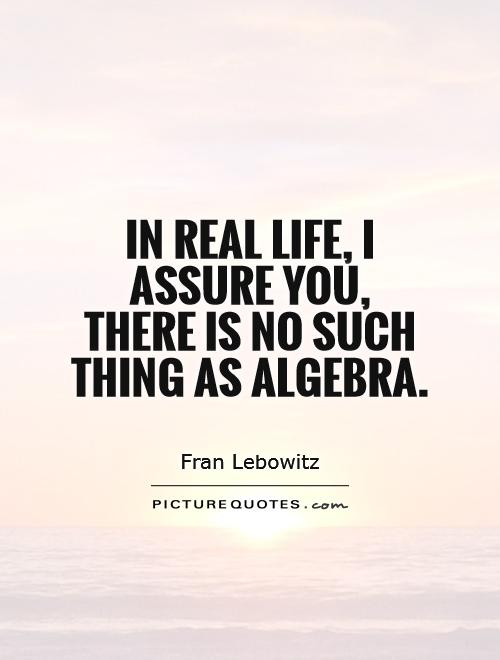
\includegraphics[scale=0.3]{will-i-use-algebra.jpg}
	\end{center}
\end{frame}

\begin{frame}
	А вот если считаем, что откидываем старшие, то получаем коммутативное кольцо с единицей $\mathbb{Z}/256\mathbb{Z}$.

	\begin{center}
		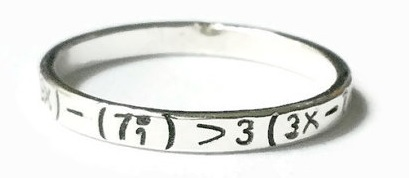
\includegraphics[scale=0.5]{math-ring.jpg}
	\end{center}

	\begin{itemize}
		\item
			По сути "--- просто арифметика, где все числа берутся по модулю 256.
		\item
			Сложение, вычитание, умножение в таких объектах прекрасно определены и непротиворечивы.
		\item
			Можно делать что угодно, и мы всегда получим корректный результат по модулю 256.
		\item
			В железе реализовать просто "--- считаем только последние 8 бит результата.
	\end{itemize}
\end{frame}

\begin{frame}{Деление}
	С делением хуже (деление "--- обратное к умножению).

	После взятия по модулю иногда можно однозначно восстановить ответ, а иногда нет (на алгебре расскажут, когда):
	\begin{align*}
	    34 / 17 &= 2 \\
		4386 / 17 &= 258 = 2 \mod 256 \\
		48 / 4 &= 12 \\
		\underbrace{(256+48)}_{304} / 4 &= 76
	\end{align*}
	Поэтому деление всегда считает, что у нас числа помещаются в 8 бит, и делим мы с остатком.
\end{frame}

\subsection{Знаковые числа}

\begin{frame}
	\tableofcontents[currentsection,currentsubsection]
\end{frame}

\begin{frame}
	Можно сказать, что в первом бите храним знак (прямой код).
	Тогда надо разбирать случаи в процессоре для всех операций и сравнения.
	Появляются $+0$ и $-0$, так что ещё и сравнение на равенство сильно менять.

	А можно сказать, что:
	\begin{align*}
		x &= x + 256 \mod 256 \\
		-56 &= -56 + 200 = 200 \mod 256
	\end{align*}
	Самое главное свойство числа $-x$ "--- это $(-x)+x=0$!.
\end{frame}

\begin{frame}
	\begin{center}
		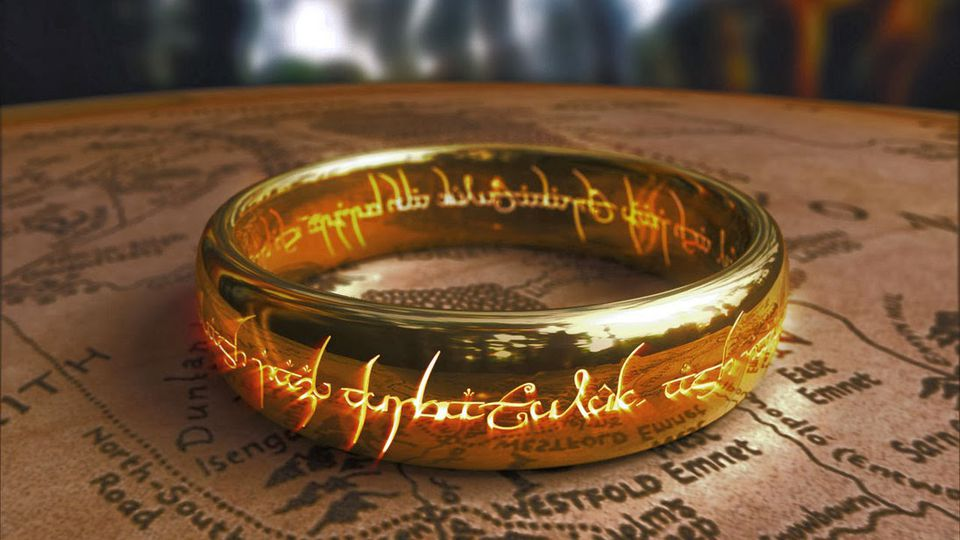
\includegraphics[scale=0.3]{one-ring-to-rule.jpg}
	\end{center}
\end{frame}

\begin{frame}
	Алгебра говорит, что $-x$ "--- это \textit{обратный по сложению к $x$}.
	В кольцах он есть.

	Мы только поменяли, как мы интерпретируем числа, но не их битовую запись:
	\[
		-56 + 100 = -56 + 256 + 100 = 200 + 100 = \t{1100 1000} + \t{0110 0100} = \t{1 0010 1100} = \t{0010 1100} = 44
	\]
	Таким образом, сложение, вычитание, и даже умножение по-прежнему работают (спасибо алгебраистам, что доказали).
	Упражнение: проверить.

	С делением хуже:
	\[
		-10 / 5 = (256 - 10) / 5 = 246 / 5 = 49.5 = \t{???}
	\]
\end{frame}

\begin{frame}{Стандартная конвенция}
	Обычно разделяют отрезок ровно пополам: $[-128; 127]$.
	Тогда по самому старшему биту определяют знак: 1 "--- отрицательное, 0 "--- неотрицательное.
	Такая конвенция называется дополнительный код: отрицательное и положительно число в сумме дают нули или
	дополняют до степени двойки $2^8$.

	Надо разбирать случаи в сравнении чисел и в делении с остатком (поэтому они в ассемблере появляются знаковые/беззнаковые).

	Операция смены знака: инвертировать все биты и добавить единицу, так как инвертация бит "--- вычитание из \t{1111 1111} (255).

	Упражнение: как представлены -1, -128, 127, 128?
	128 никак не представлено, есть некоторая асимметрия.
	Что будет, если мы возьмём $-(-128)$?
\end{frame}

\subsection{Порядок байт}

\begin{frame}
	\tableofcontents[currentsection,currentsubsection]
\end{frame}

\begin{frame}{Играем в игру}
	Напоминание: порядок бит в байте мы из программы никак не определим, на картинке рисуем слева старшие, справа младшие.

	Порядок байт в памяти "--- слева меньшие адреса, справа большие.

	\begin{center}
		\pause
		\begin{tabular}{|c|c|c|c|l|}
			\hline
			\multicolumn{4}{|c|}{Адрес} & Значение \\
			 & 2 & 3 & & \\\hline
			\dots & \t{0000 0001} & \t{0000 0011} & \dots & \pause 259 \\\noalign{\pause}
			\dots & \t{0000 0001} & \t{0000 0011} & \dots & \pause 769 \\
			\hline
		\end{tabular}
		\pause
	\end{center}

	\begin{itemize}
		\item
			В каком порядке идут байты в памяти?
			Они же тоже бывают старшие и младшие.
		\item
			Как договорились "--- так и идут.
			Договариваются по-разному на разных процессорах и в разных протоколах.
		\item
			Свойство <<порядок байт>> называется endianness.
	\end{itemize}
\end{frame}

\begin{frame}

	\begin{center}
		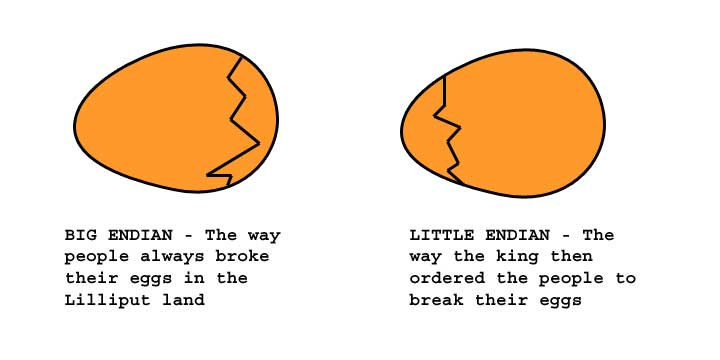
\includegraphics[scale=0.3]{eggs.jpg}
	\end{center}

	Есть два клана: little-endian (остроконечники) и big-endian (тупоконечники).
	По-русски всегда используют английские термины.
\end{frame}

\begin{frame}{Big-endian}
	Используется в низкоуровневых сетевых протоколах (TCP) и процессорах Atmel AVR (ATmega и прочие).

	Младший байт имеет больший адрес.
	Читается просто:
	\begin{center}
		\begin{tabular}{|c|c|c|c|l|}
			\hline
			\multicolumn{4}{|c|}{Адрес} & Значение \\
			& 2 & 3 & & \\\hline
			\dots & \t{0000 0001} & \t{0000 0011} & \dots & $\t{0000~00\textbf{01}~0000~00\textbf{11}}_2=259_{10}$ \\
			\hline
		\end{tabular}
	\end{center}

	Надо очень аккуратно помнить адрес и размер числа:
	\begin{center}
		\begin{tabular}{|c|c|c|l|}
			\hline
			\multicolumn{3}{|c|}{Адрес} & Значение \\
			& 2 & & \\\hline
			\dots & \t{0000 0001} & \dots & $\t{0000 0001}_2=1_{10}$ \\
			\hline
		\end{tabular}
	\end{center}
\end{frame}

\begin{frame}{Little-endian}
	Используется в x86: <<младший байт имеет меньший адрес>>.

	Читается хуже:
	\begin{center}
		\begin{tabular}{|c|c|c|c|l|}
			\hline
			\multicolumn{4}{|c|}{Адрес} & Значение \\
			& 2 & 3 & & \\\hline
			\dots & \t{0000 0001} & \t{0000 0011} & \dots & $\t{0000~00\textbf{11}~0000~00\textbf{01}}_2=769_{10}$ \\
			\hline
		\end{tabular}
	\end{center}
	Если только мы не Intel и не пишем к этому документацию:
	\begin{center}
		\begin{tabular}{|c|c|c|c|l|}
			\hline
			\multicolumn{4}{|c|}{Адрес} & Значение \\
			& \textbf{3} & \textbf{2} & & \\\hline
			\dots & \t{0000 0011} & \t{0000 0001} & \dots & $\t{0000~0011~0000~0001}_2=769_{10}$ \\
			\hline
		\end{tabular}
	\end{center}
	Они у себя всё пишут от старших к младшим: байты с меньшими адресами справа, младшие биты справа.
\end{frame}

\begin{frame}{Особенности Little-endian-1}
	Можно почти безболезненно конвертировать между типами:
	\begin{center}
		\begin{tabular}{|c|c|c|c|r|l|}
			\hline
			\multicolumn{4}{|c|}{Адрес} & \multicolumn{2}{|c|}{Значение} \\
			& 2 & 3 & & & \\\hline
			\dots & \t{0000 0011} & \t{0000 0001} & \dots & $\t{0000~0001~0000~0011}_2$ & $259_{10}$ \\
			\dots & \t{0000 0011} & \dots         & \dots & $\t{0000~0001}_2$           & $3_{10}$ \\
			\dots & \t{0000 0101} & \t{0000 0000} & \dots & $\t{0000~0000~0000~0101}_2$ & $5_{10}$ \\
			\dots & \t{0000 0101} & \dots         & \dots & $\t{0000~0101}_2$           & $5_{10}$ \\
			\dots & \t{1111 0011} & \t{0000 0000} & \dots & $\t{0000~0000~1111~0011}_2$ & $243_{10}$ \\
			\dots & \t{1111 0011} & \dots         & \dots & $\t{1111~0011}_2$           & $243_{10}$ \\
			\dots & \t{1111 0011} & \dots         & \dots & $\t{1111~0011}_2$           & $-13_{10}$ \\
			\dots & \t{1111 0011} & \t{1111 1111} & \dots & $\t{1111~1111~1111~0011}_2$ & $-13_{10}$ \\
			\hline
		\end{tabular}
	\end{center}
\end{frame}

\begin{frame}[t]{Особенности Little-endian-2}
	\begin{itemize}
		\item
			Есть проблема со знаком, если мы переходим от меньшего типа к большему.
		\item
			Надо \textit{расширять знак}, если у нас было знаковое число:
			заполнять старшие байты либо нулями, либо единицами (в зависимости от\only<1>{...}\only<2->{ старшего бита в числе}).
	\only<3->{
		\item
			Если число было беззнаковое, то надо старший байт заполнить нулями.
	}
	\end{itemize}

	\only<3->{
	Компиляторы низкоуровневых языков делают это автоматически, когда вы делаете какие-то присваивания.
	Разумеется, надо аккуратно следить за типами, иначе не сделают.

	Замечание: иногда, несмотря на тип \t{int}, какие-то функции могут ожидать в нём на самом деле не число,
	а набор байт в определённом порядке.
	Яркий пример "--- номер порта в работе с сетью на C, функция \t{htons} "--- это оно.
	}
\end{frame}

\begin{frame}{Резюме}
	\begin{enumerate}
		\item
			Целые числа хранятся в двоичной системе счисления.
		\item
			Знаковость числа определяется лишь типом данных.
		\item
			Самый распространённый способ кодирования отрицательных чисел "--- <<дополнительный код>>.
		\item
			В дополнительном коде старший бит отвечает за знак, а арифметика делатеся так же, как и в беззнаковых числах.
		\item
			Операциям сравнения чисел на меньше/больше и делению важно знать, работаем ли мы в дополнительном коде или с беззнаковыми числами.
		\item
			Порядок байт в числах может отличаться даже в разных местах внутри одного приложения.
			Читайте документацию, если работаете с чем-то на уровне байт!
		\item
			Если работаете с little-endian и меняете количество байт в числе "--- позаботьтесь о знаке.
		\item
			Если есть либо дополнительный код, либо переполнения, то важно количество бит/байт в числе.
	\end{enumerate}
\end{frame}


\end{document}
